The assignment was to design a simple multi-cycle processor in VHDL.
It should then be synthesized and simulated using the logic simulation tool ModelSim[TODO ref].
Finally the design should be run and tested on the FPGA onboard a MicroBlaze-based embedded system.

\section{Instruction set}
The processor was required to follow the MIPS instruction set, with at least the following instructions implemented:
\begin{itemize}
    \item Several ALU instructions (All working on two registers and storing the result in a third):
        \begin{itemize}
            \item ADD - Addition
            \item SUB - Subtraction
            \item SLT - Test if the first source register is less than second
            \item AND - Bitwise and
            \item OR  - Logical or
        \end{itemize}
    \item BEQ - branch if registers are equal
    \item LW - Load word from memory
    \item SW - Store word to memory
    \item LUI - Store immediate value shifted left 16 bits in a register
    \item J - Jump
\end{itemize}

\section{Supplied Materials}
The following materials was supplied:
\begin{itemize}
    \item Suggested MIPS Architecture - See figure \ref{fig:sugarchi}
    \item Communication Framework - Providing an interface towards the embedded system
    \item VHDL Components - Register File, ALU and Adder
    \item Test Program - For verification of design
\end{itemize}

\begin{figure}[ht]
    \centering
    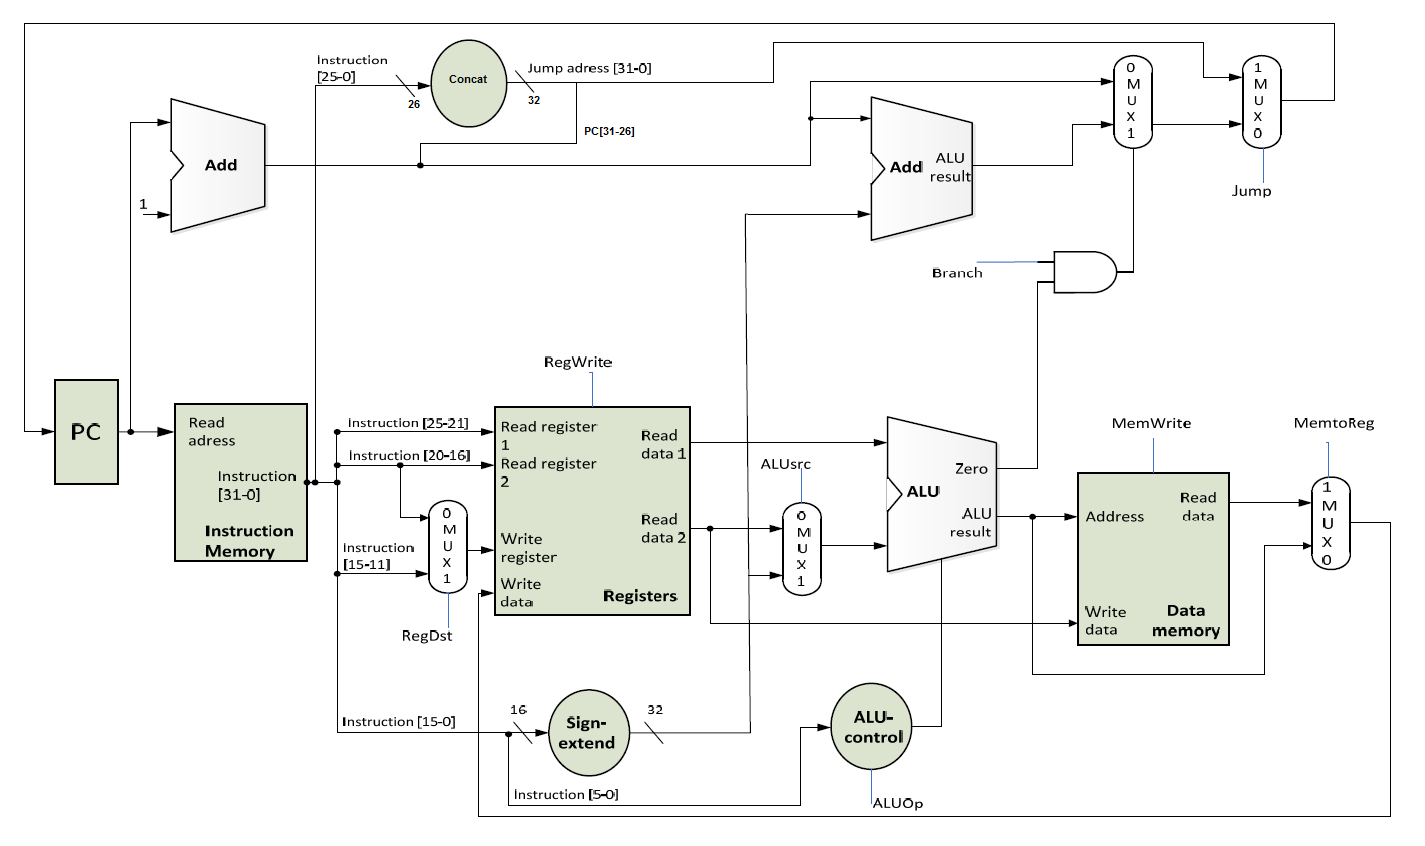
\includegraphics[scale=0.3]{figures/suggestedarchitecture.png}
    \caption{\label{fig:sugarchi}Suggested Architecture.}
\end{figure}

\section{Suggestions}
It was suggested to use a state machine with the states Fetch, Execute and Stall, where Fetch would retrieve the instruction from memory and Execute would run the instruction. Stall would only be needed in case of data memory access.
